%%%%%%%%%%%%%%%%%%%%%%%%%%%%%%%%%%%%%%%%%%%%%%%%%%%%%%%%%%%%%%%%
% %
% Seth Cram %
% ECE351 Section 53 %
% Lab 9 %
% Due 03/29/2022 %
% Any other necessary information needed to navigate the file %
%
%
% %
%%%%%%%%%%%%%%%%%%%%%%%%%%%%%%%%%%%%%%%%%%%%%%%%%%%%%%%%%%%%%%%%
%%%%%%%%%%%%%%%%%%%%%%%%%%%%%%%%%%%%%%%%%%%
%%% DOCUMENT PREAMBLE %%%
\documentclass[12pt]{report}
\usepackage[english]{babel}
%\usepackage{natbib}
\usepackage{url}
\usepackage[utf8x]{inputenc}
\usepackage{amsmath}
\usepackage{graphicx}
\graphicspath{{images/}}
\usepackage{parskip}
\usepackage{fancyhdr}
\usepackage{vmargin}
\usepackage{listings}
\usepackage{hyperref}
\usepackage{xcolor}
\usepackage{verbatim}
\usepackage{listings}

\definecolor{codegreen}{rgb}{0,0.6,0}
\definecolor{codegray}{rgb}{0.5,0.5,0.5}
\definecolor{codeblue}{rgb}{0,0,0.95}
\definecolor{backcolour}{rgb}{0.95,0.95,0.92}

\begin{comment} %have to use verbatim package for this

\section{Personal Notes}
            


\end{comment}

\lstdefinestyle{mystyle}{
    backgroundcolor=\color{backcolour},   
    commentstyle=\color{codegreen},
    keywordstyle=\color{codeblue},
    numberstyle=\tiny\color{codegray},
    stringstyle=\color{codegreen},
    basicstyle=\ttfamily\footnotesize,
    breakatwhitespace=false,         
    breaklines=true,                 
    captionpos=b,                    
    keepspaces=true,                 
    numbers=left,                    
    numbersep=5pt,                  
    showspaces=false,                
    showstringspaces=false,
    showtabs=false,                  
    tabsize=2
}
 
\lstset{style=mystyle}

\setmarginsrb{3 cm}{2.5 cm}{3 cm}{2.5 cm}{1 cm}{1.5 cm}{1 cm}{1.5 cm}

\title{Lab 9}		%TITLE						
% Title
\author{ Seth Cram}						
% Author
\date{03/29/2022}
% Date

\makeatletter
\let\thetitle\@title
\let\theauthor\@author
\let\thedate\@date
\makeatother

\pagestyle{fancy}
\fancyhf{}
\rhead{\theauthor}
\lhead{\thetitle}
\cfoot{\thepage}
%%%%%%%%%%%%%%%%%%%%%%%%%%%%%%%%%%%%%%%%%%%%
\begin{document}

%%%%%%%%%%%%%%%%%%%%%%%%%%%%%%%%%%%%%%%%%%%%%%%%%%%%%%%%%%%%%%%%%%%%%%%%%%%%%%%%%%%%%%%%%

\begin{titlepage}
	\centering
    \vspace*{0.5 cm}
   % \includegraphics[scale = 0.075]{bsulogo.png}\\[1.0 cm]	% University Logo
\begin{center}    \textsc{\Large   ECE 351 - 53 }\\[2.0 cm]	\end{center}% University Name
	\textsc{\Large Fast Fourier Transform }\\[.5 cm]				% Course Code
	\rule{\linewidth}{0.2 mm} \\[0.4 cm]
	{ \huge \bfseries \thetitle}\\
	\rule{\linewidth}{0.2 mm} \\[1.5 cm]
	
	\begin{minipage}{0.4\textwidth}
		\begin{flushleft} \large
		%	\emph{Submitted To:}\\
		%	Name\\
          % Affiliation\\
           %contact info\\
			\end{flushleft}
			\end{minipage}~
			\begin{minipage}{0.4\textwidth}
            
			\begin{flushright} \large
			\emph{Submitted By :} \\
			Seth Cram  
		\end{flushright}
           
	\end{minipage}\\[2 cm]
	
\end{titlepage}

%%%%%%%%%%%%%%%%%%%%%%%%%%%%%%%%%%%%%%%%%%%%%%%%%%%%%%%%%%%%%%%%%%%%%%%%%%%%%%%%%%%%%%%%%

\tableofcontents
\pagebreak

%%%%%%%%%%%%%%%%%%%%%%%%%%%%%%%%%%%%%%%%%%%%%%%%%%%%%%%%%%%%%%%%%%%%%%%%%%%%%%%%%%%%%%%%%
\renewcommand{\thesection}{\arabic{section}}

\section{Introduction}

The goal of lab 9 is to become familiar with fast Fourier transforms using Python in the Spyder IDE.

\section{Equations}
    \begin{equation}
       x_1(t) = cos(2*\pi*t) 
    \end{equation}
    \begin{equation}
       x_2(t) = 5sin(2*\pi*t) 
    \end{equation}
    \begin{equation}
       x_3(t) = 2cos((2*\pi*t) -2) + sin^2((2*\pi*t)+3)
    \end{equation}
    
\section{Methodology}

%This section will describe how you went about solving the lab. Make sure you go into detail about any method you used. %Include coding samples here if necessary. This is also where you would include necessary derivations. An example of %inserting code into the report is given. Do not go overboard on inserting code into your report, only use whats %absolutely necessary to illustrate your point.

    \paragraph{} First, I created the user-defined Fast Fourier Transform (fft) function that executed the code given in the lab handout. My contribution to creating the function involved the values returned. I returned the magnitude, phase, and frequency as a tuple. 
    \paragraph{} Second, I plotted $x_1(t)$. Then, in the same figure, I plotted the magnitude and phase as separate plots. Referencing the lab handout appendix, I also created two other magnitude and phase plots that limited the x-values to focus on important aspects of the function. I repeated this process for $x_2(t)$ and $x_3(t)$. 
    \paragraph{} Thirdly, I duplicated my fft function and added some code to clean it up. As mentioned in the lab handout, I eliminated all the small phase magnitudes. I then reran the code for the first three plots and received their clean versions. 
    \paragraph{} Finally, I needed to use my fft function on the Fourier series approximation of a square wave plotted in Lab 8. Using only the N = 15 and T = 8 case, I ran my Lab 8 function results through my fft function. I then generated the same type of plot as previously seen in the lab.   
    
\section{Results}

%This section will go over the results of the lab. Use this area to describe %if the lab worked as expected or if the results are unexpected or different %from your hand calculations or intuition. Part of being a good engineer is %gaining intuition about these problems and being able to understand quickly %if something is wrong. Use code, plots, tables, and figures as necessary. %Make sure to cite all other works used and note them in the bibliography. A %sample entry is in this document.
    
    \paragraph{} Initially, I didn't have many expectations since I didn't write the internals of the fft function. But, I did have intrinsic knowledge regarding cosine and sine functions, so I expected them to be about 90 degrees out of phase wrt to one another. I plotted from 0 to 2 seconds, used the output frequency, and finally from -2 to 2 to grab the most important values.    
    
    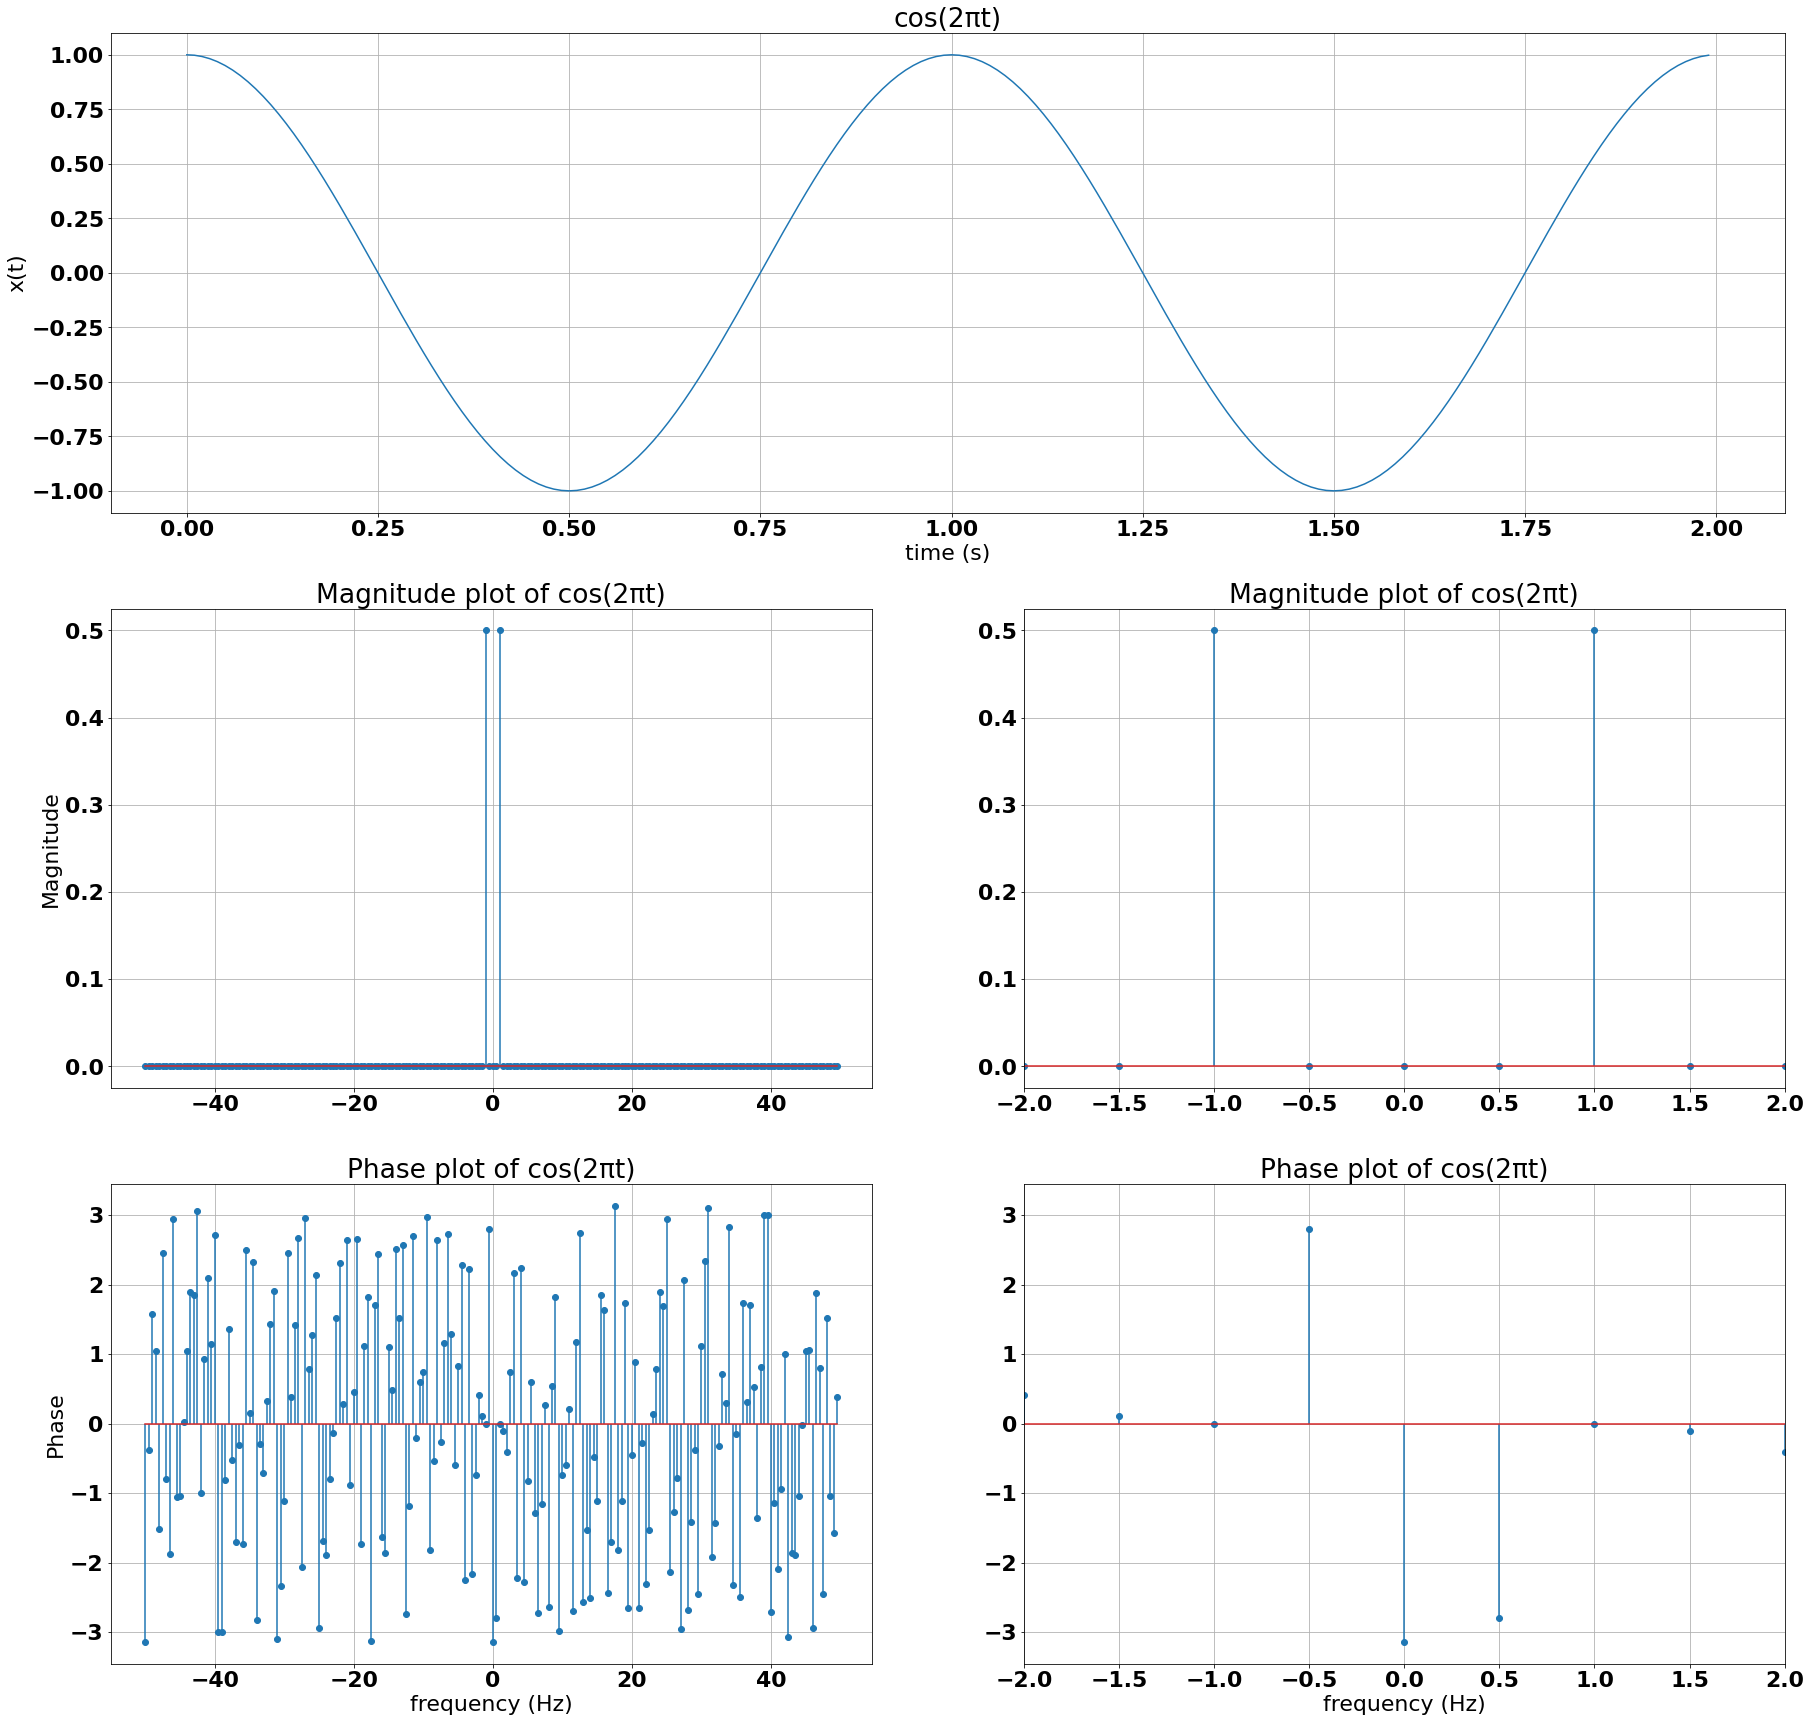
\includegraphics[scale=0.25]{Figure 2022-03-22 205111 (0).png}
    
    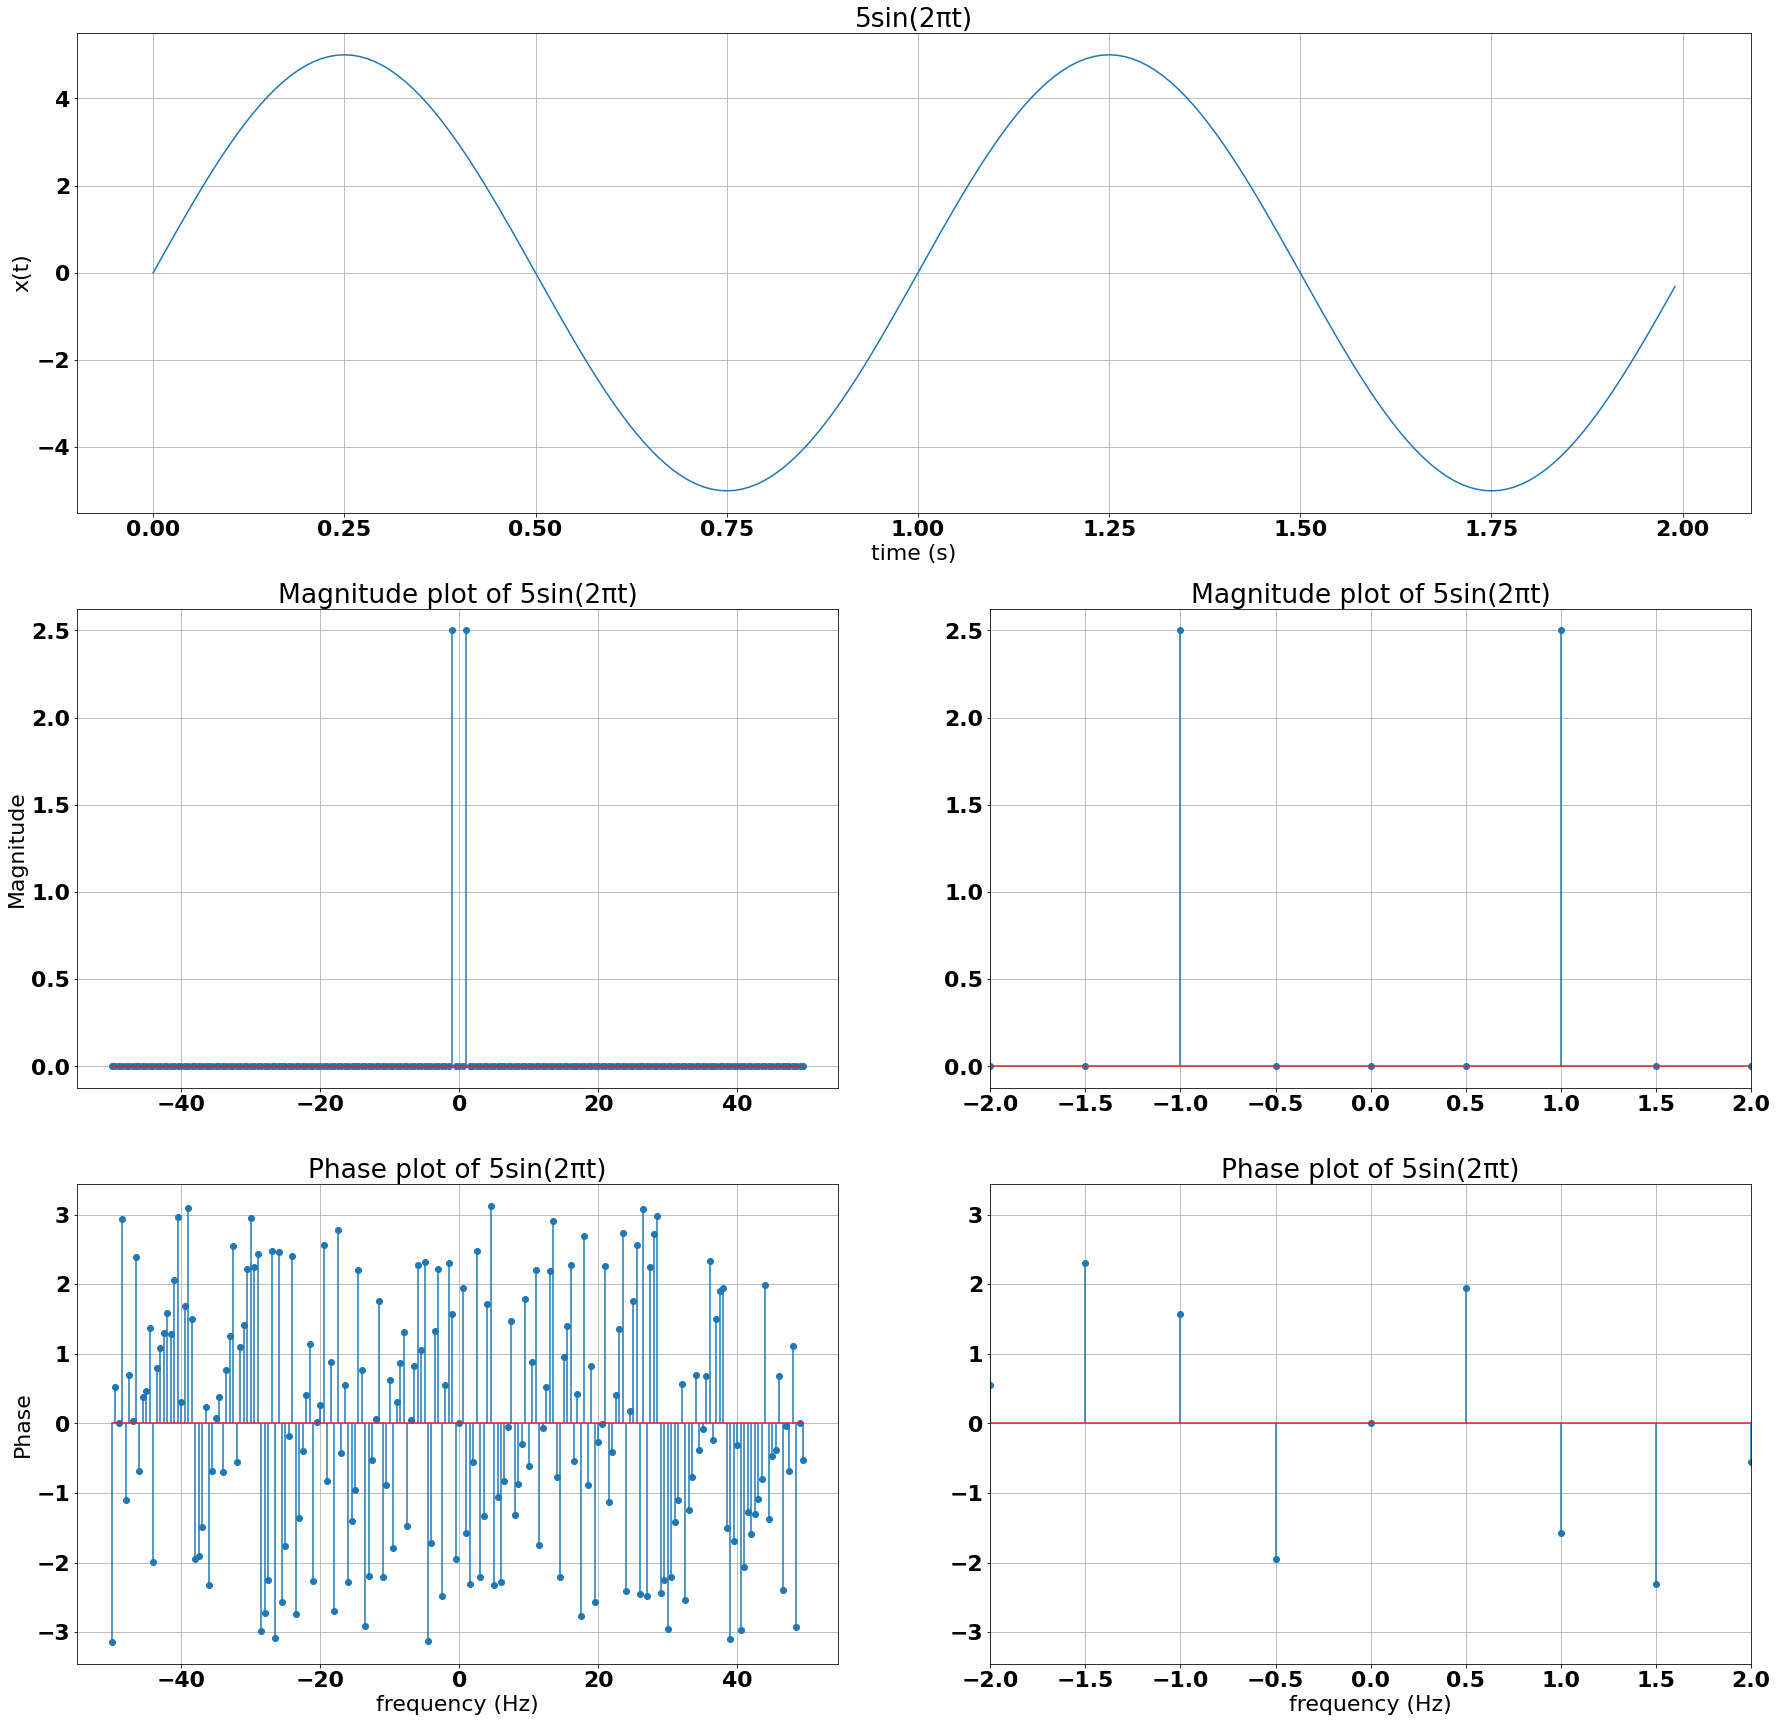
\includegraphics[scale=0.25]{Figure 2022-03-22 205111 (1).png}
    
    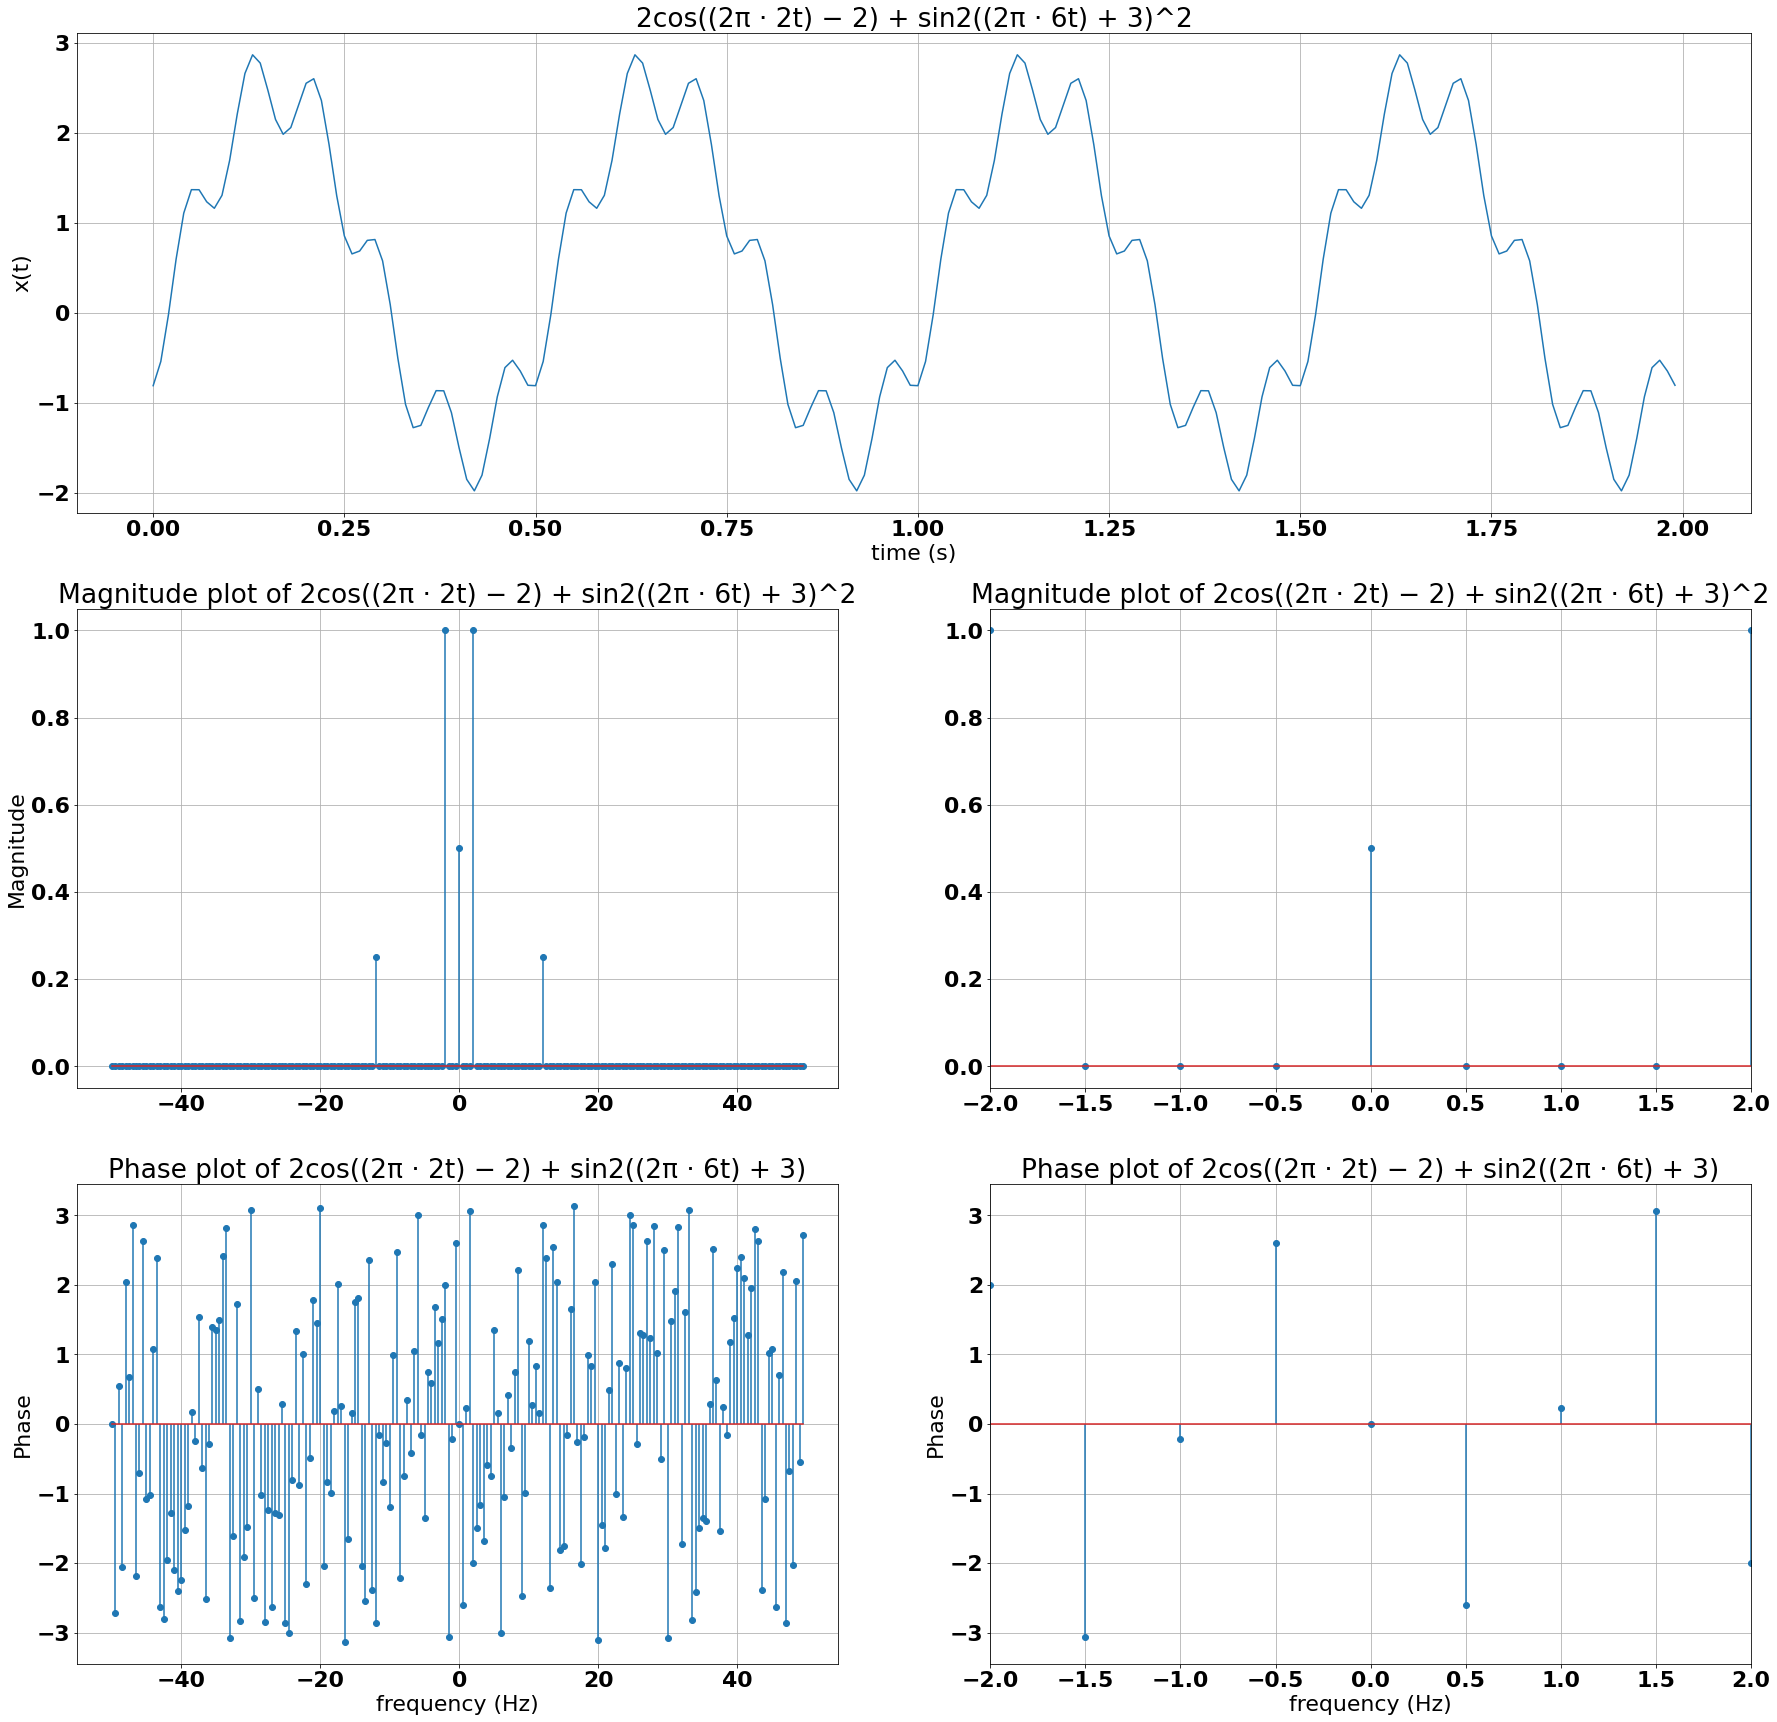
\includegraphics[scale=0.25]{Figure 2022-03-22 205111 (2).png}
    
    \paragraph{} As seen above, it's rather hard to tell if my expectations held true or not. The sine and cosine functions definitely output different phases, but with all the noise it's hard to say how different they are. 
    
    \paragraph{} My expectations for the clean functions was that they'd be exactly like the functions above, except with less noise and more clearly defined outputs. 
    
    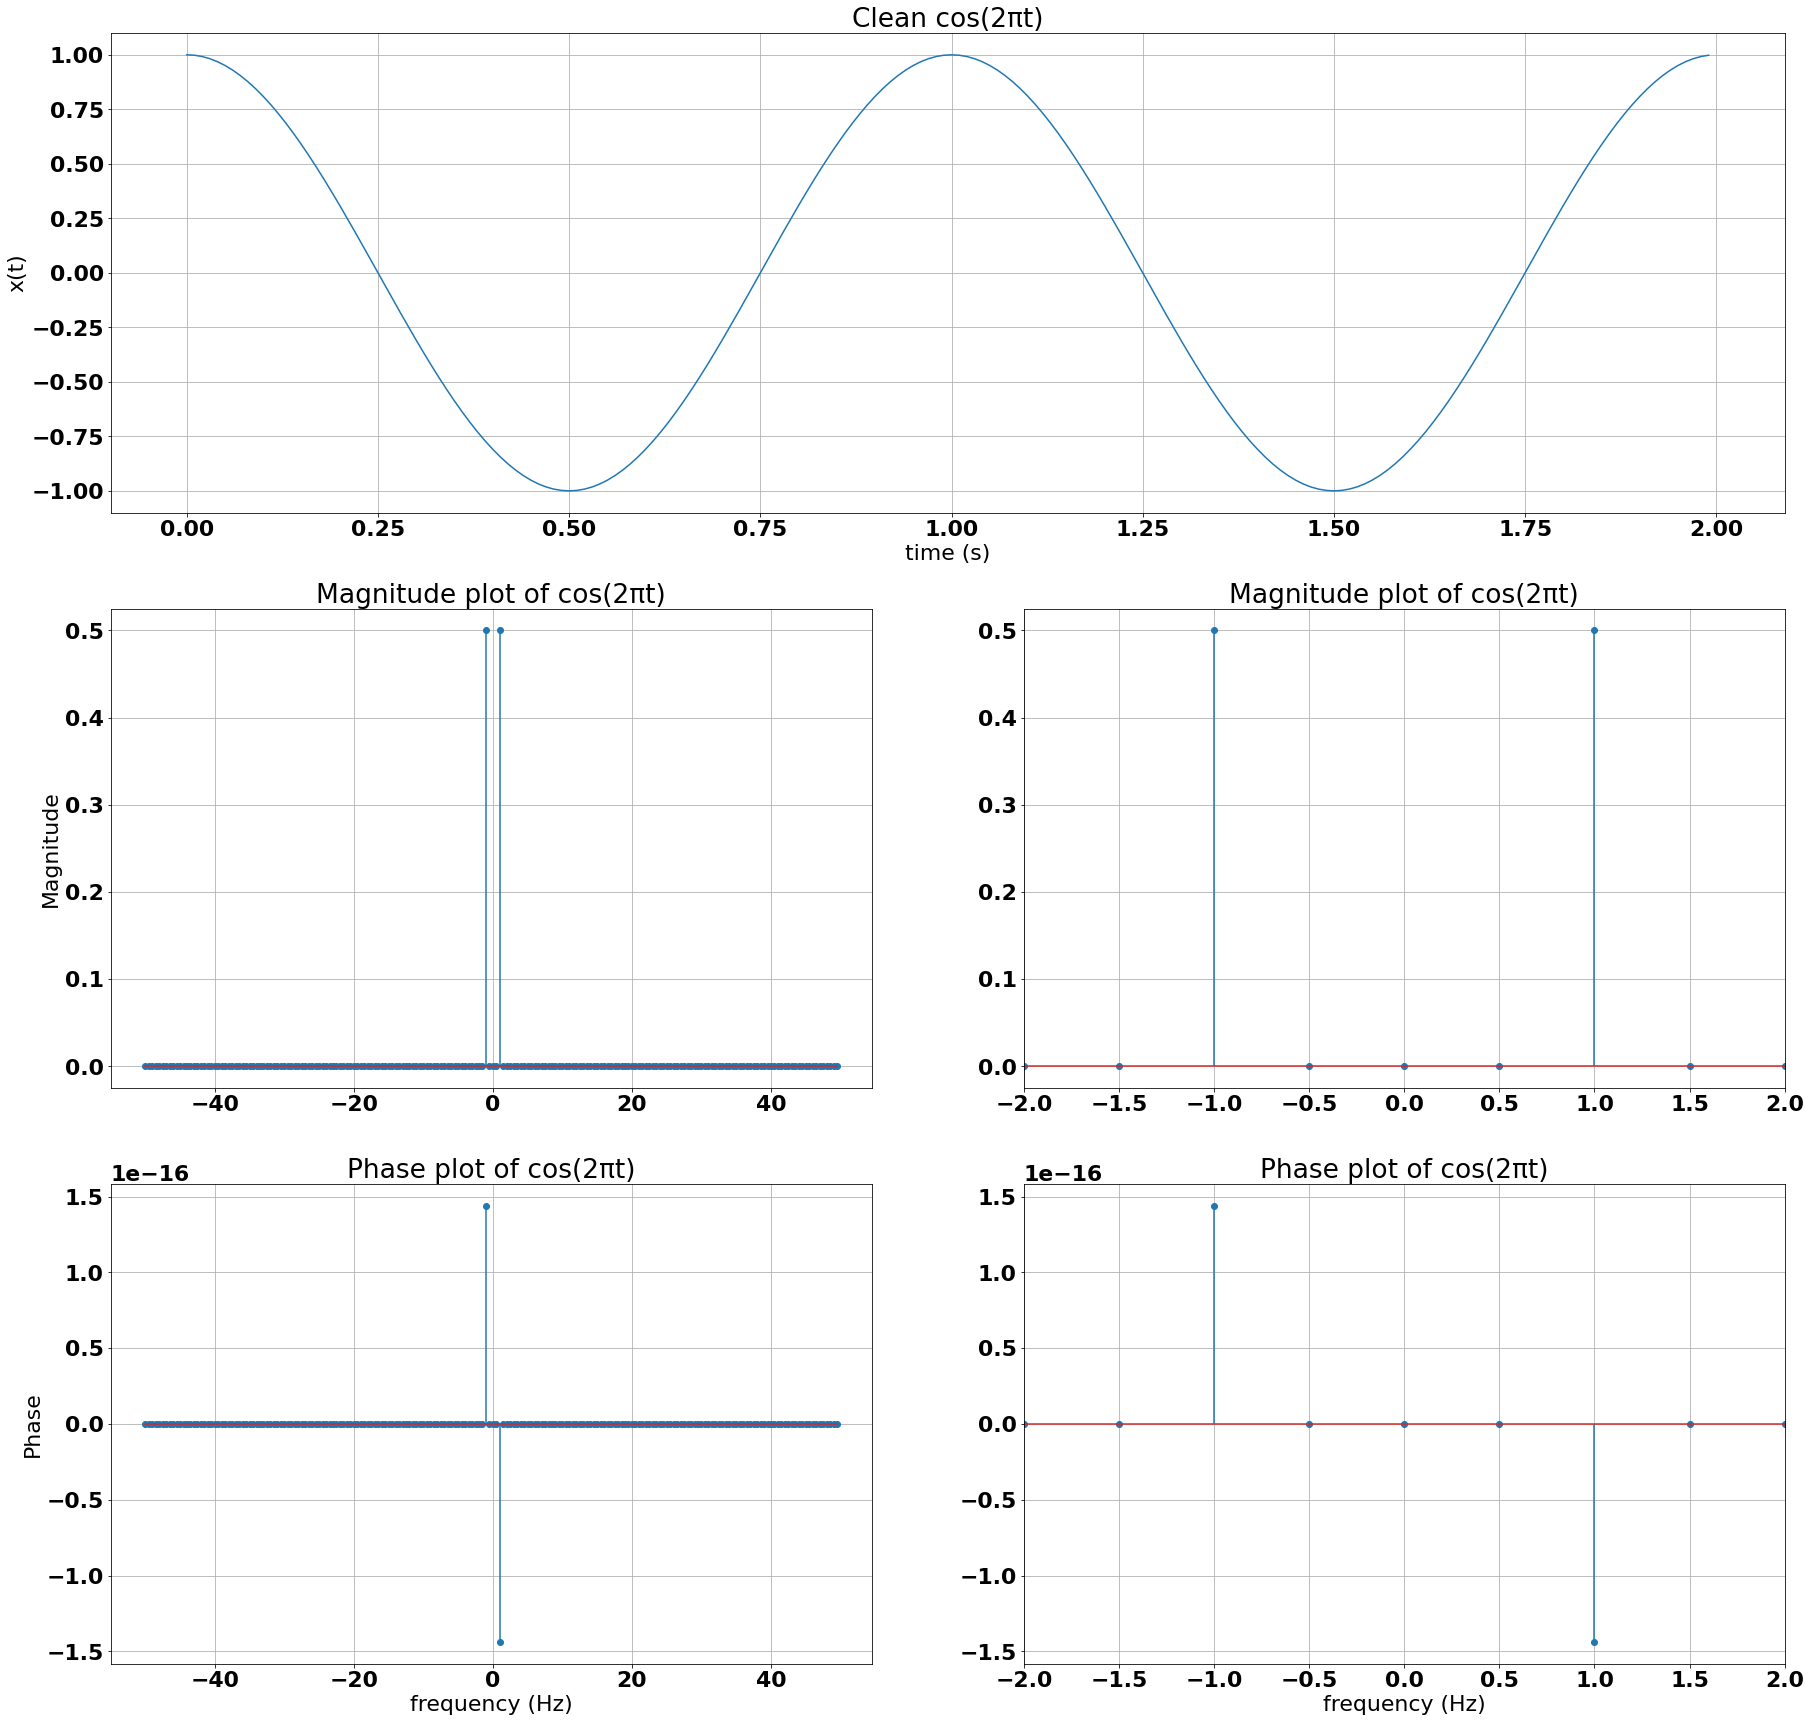
\includegraphics[scale=0.25]{Figure 2022-03-22 205111 (3).png}
    
    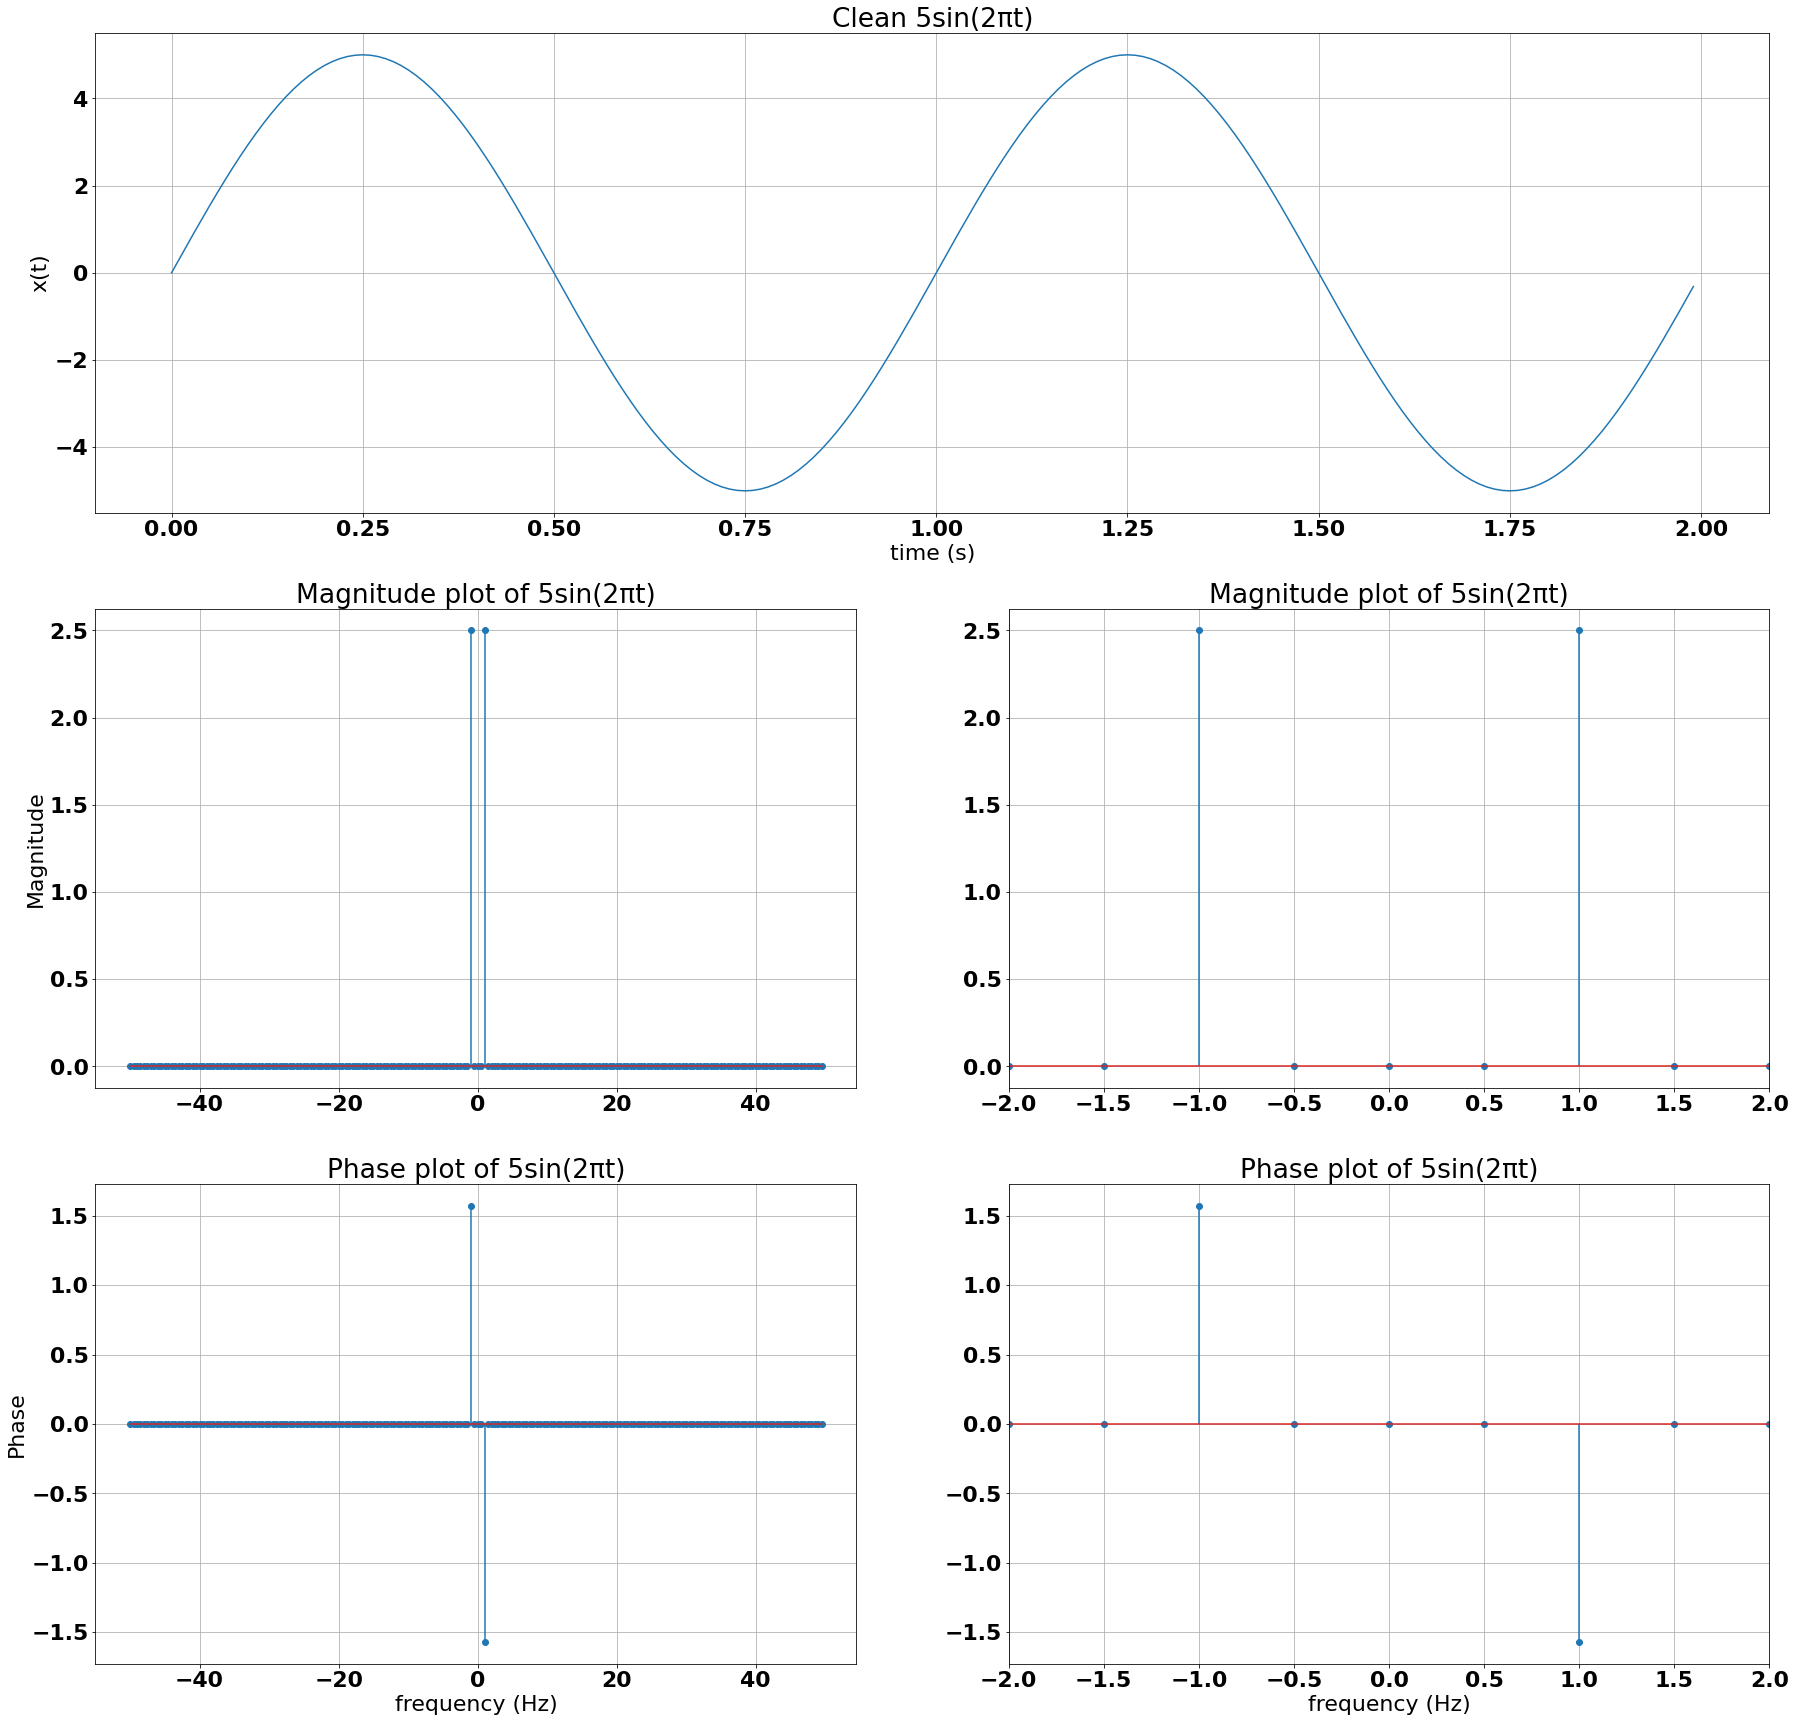
\includegraphics[scale=0.25]{Figure 2022-03-22 205111 (4).png}
    
    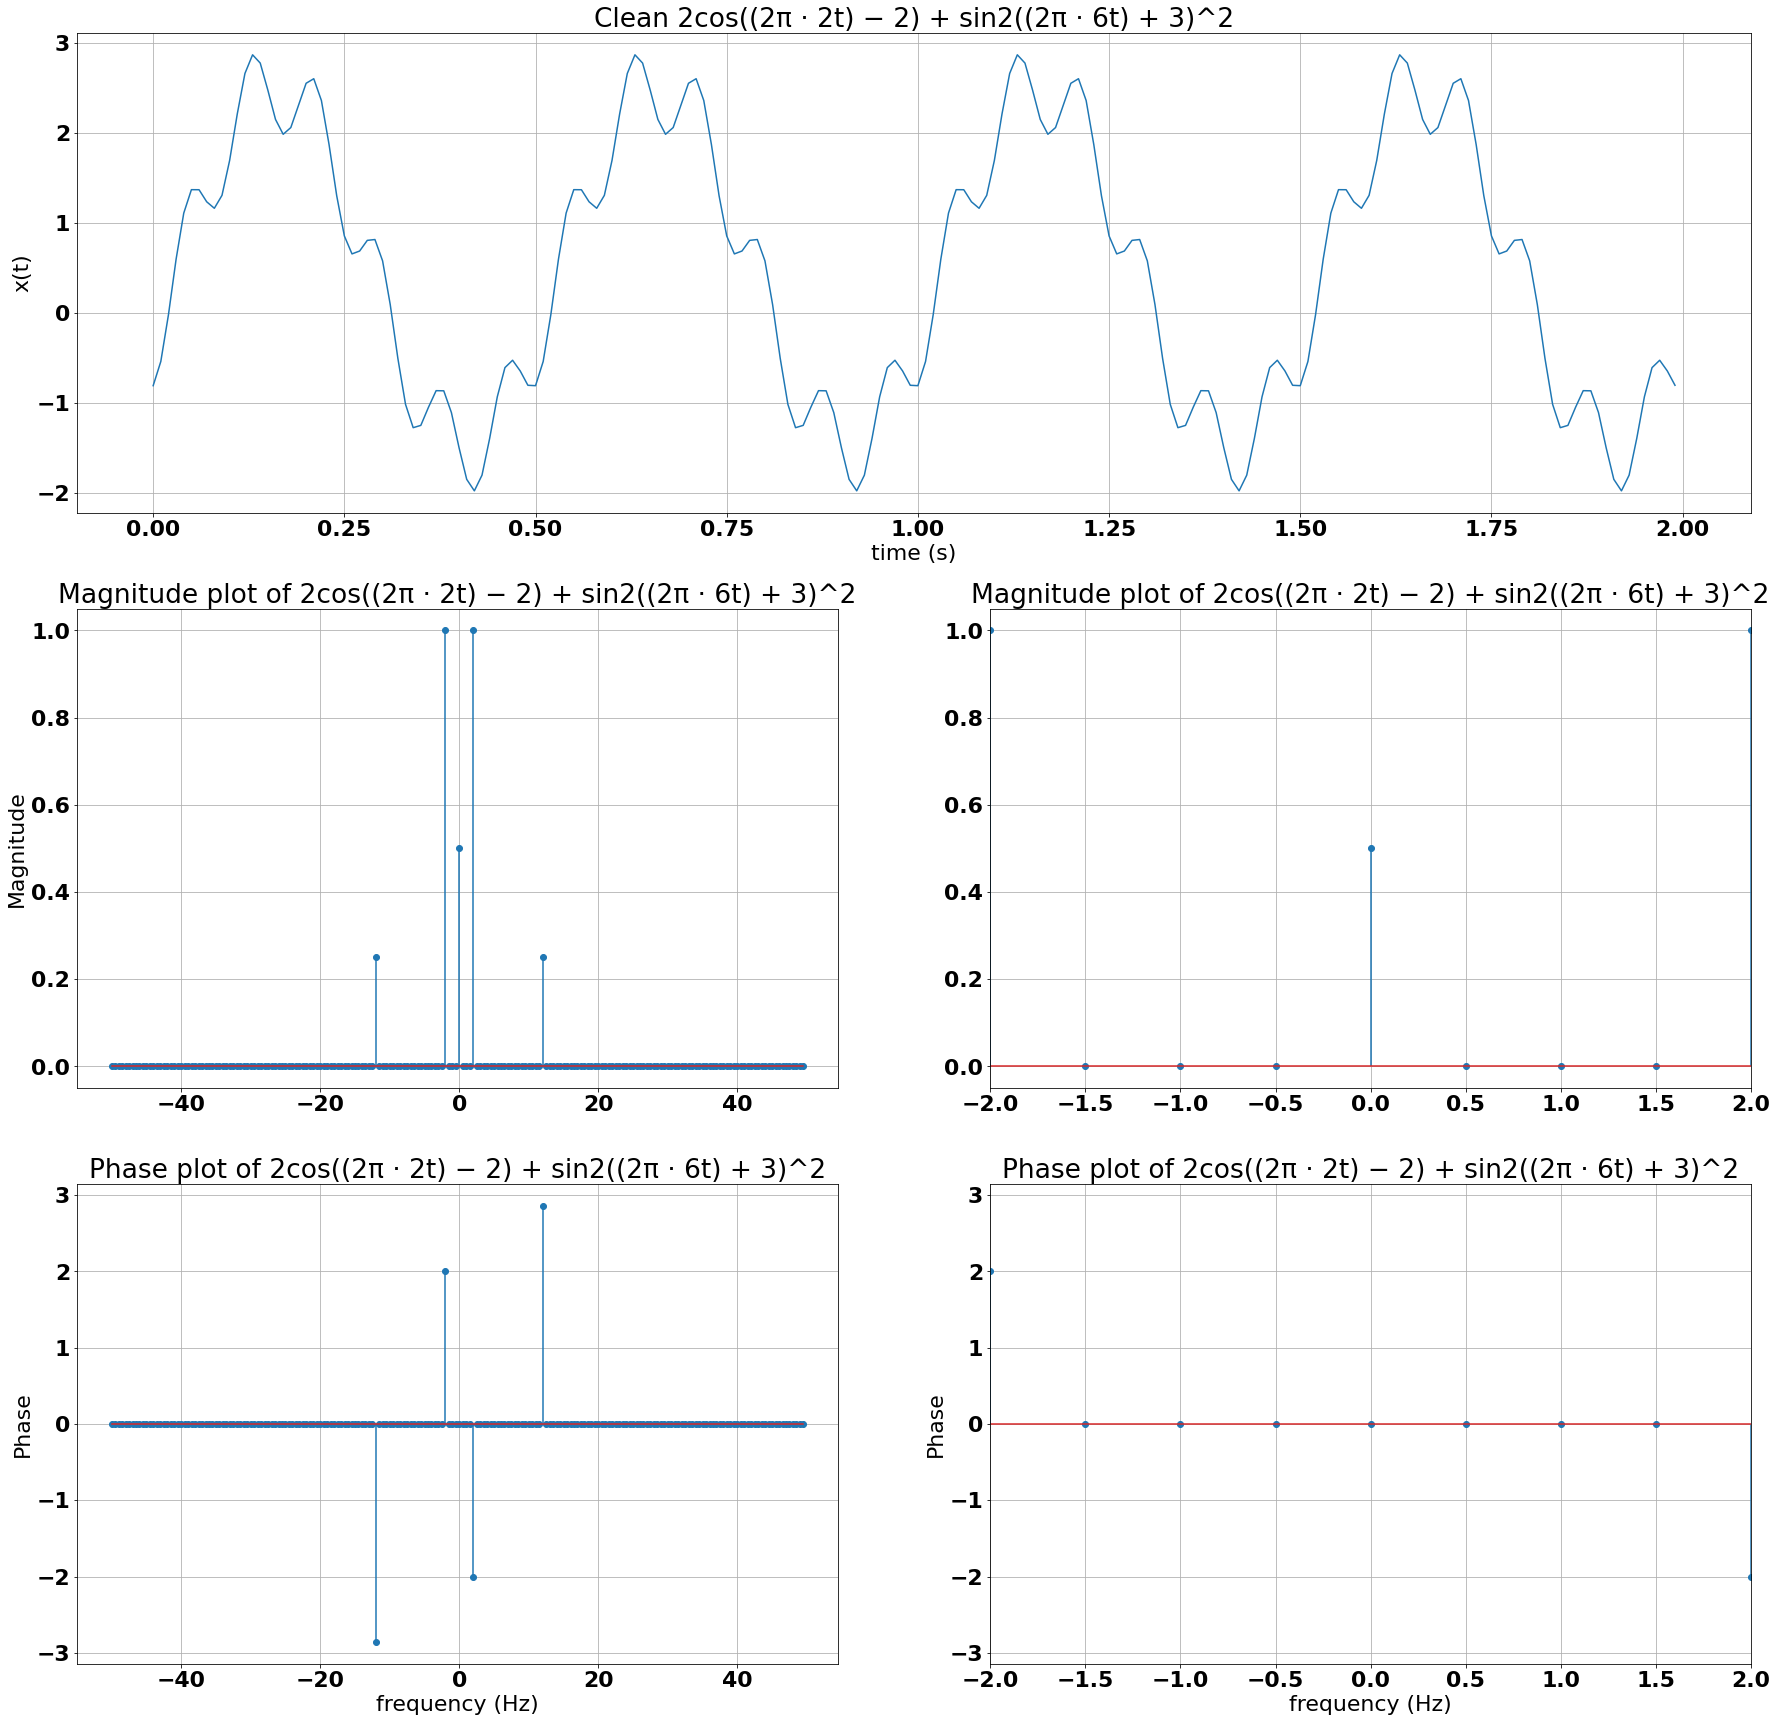
\includegraphics[scale=0.25]{Figure 2022-03-22 205111 (5).png}
    
    \paragraph{} As seen above, there's far less noise in our cleaned up graphs. As a result, we can now make the judgement call that my expectations held before we ever started plotting are incorrect. As seen in the bottom right of both the sine and cosine functions, the phases are the exact same, not 90 degrees out of phase. I'm not entirely sure why this is the case. 
    
    \paragraph{} My expectation for the Fourier series approximated square wave was that since we're only iterating up to N=15, it'd be fairly noisy since our cleaned up function only gets rid of noise that's close to zero.  
    
    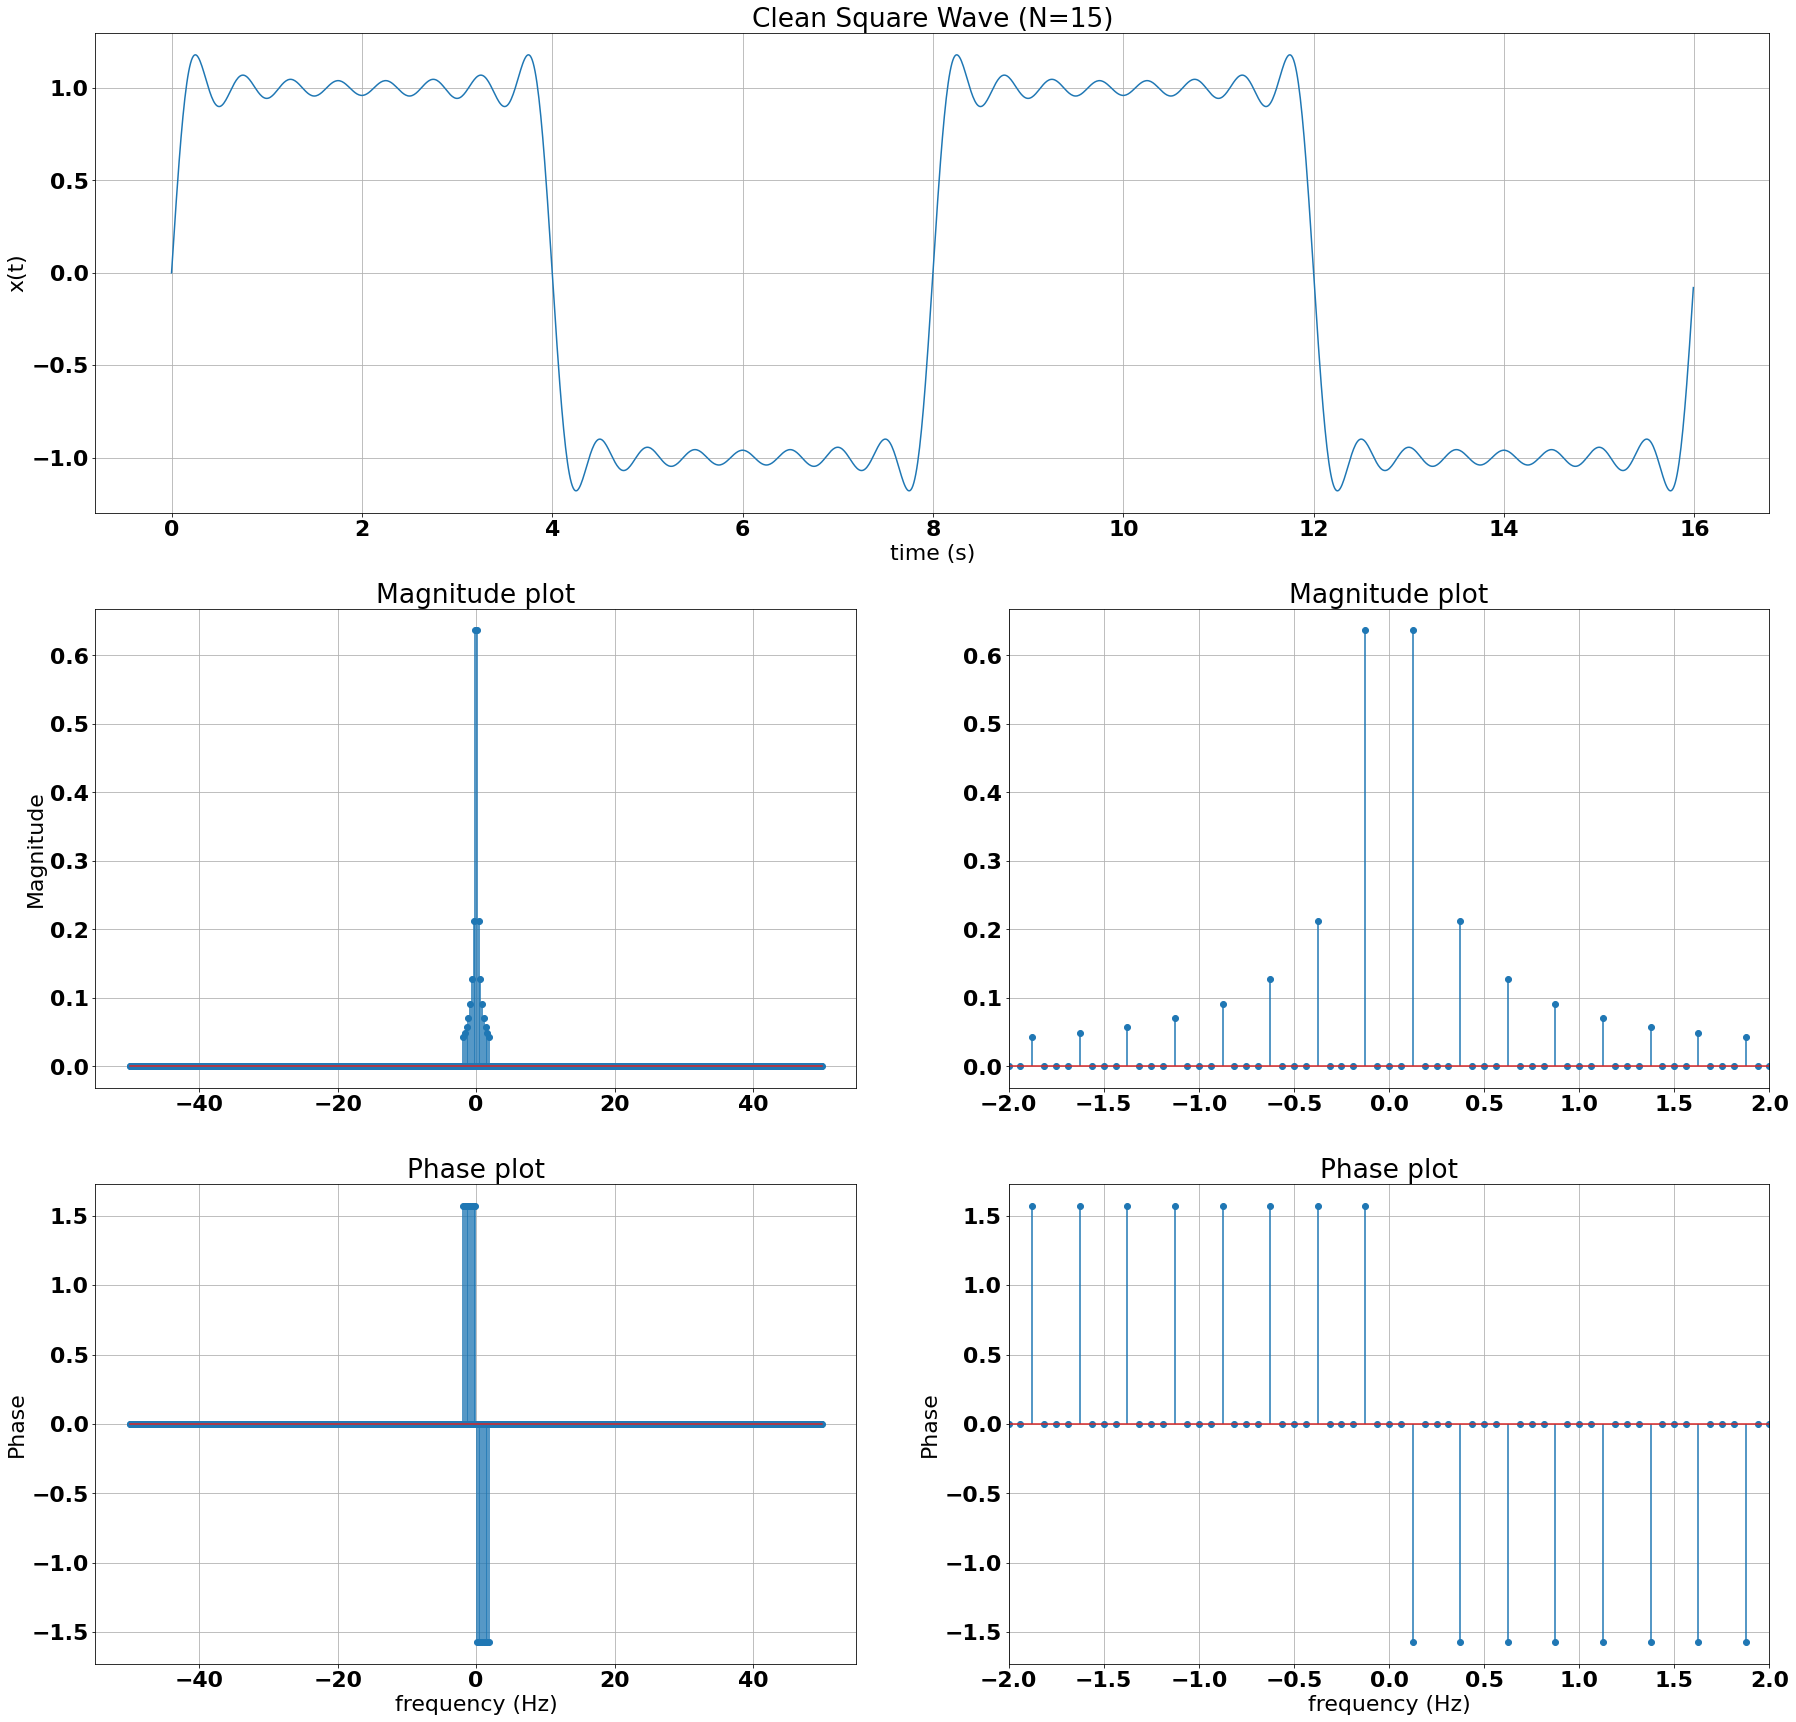
\includegraphics[scale=0.25]{Figure 2022-03-22 205111 (6).png}

    \paragraph{} As seen above, my expectation held true with quiet a bit of noise present in both the magnitude and phase graphs. 

\section{Error Analysis}

%This section will discuss error analysis of the experiment. Since this lab %deals with ideal simulation there shouldn't be any sources of error, so %instead this section can be used to describe any difficulties you had during %lab and how you solved them. Alternatively, if you couldn't get the %experiment to work, which is okay, you need to use this section to explain why %you couldn't get it to work to earn full points. 

\paragraph{} The main difficulty I encountered was getting the graphs to line up properly. Lab 9 was the first time I've had to use subplots both vertically and horizontally on one figure. The documentation also wasn't very clear on the usage.  

\paragraph{} A possible source of error comes from how a fft does fourier series in steps, so we just throw away a chunk of data. So, a fft shouldn't be expected to be nearly as precise as a normal Fourier transform, but I can imagine some uses for such approximation.    

\section{Questions} %also address any deliverables not yet put in yet
    \begin{enumerate}
        \item  What happens if fs is lower? If it is higher? fs in your report must span a few orders of magnitude
        \paragraph{} If fs is lower, the functions are much less accurate, but more noise is removed as a result from the unclean versions since not as many steps are taken. If fs is higher, the functions are much more accurate, but we get far more noise in the unclean versions. Therefore, since we're filtering for noise, a higher fs should be preferred since it's more accurate.  
        
        \item What difference does eliminating the small phase magnitudes make?
        \paragraph{} Eliminating the small phase magnitudes, as seen in our three clean graphs, cleans up almost all of the excess noise. It helps us focus on the important aspects and areas of our graph while ignoring minor variation.  
        
        \item Verify your results from Tasks 1 and 2 using the Fourier transforms of cosine and sine. Explain why your results are correct. You will need the transforms in terms of Hz, not rad/s. For example, the Fourier transform of cosine (in Hz) is:
            $F\{cos (2\pi f_0t)\} = \frac{1}{2}[\delta(f − f_0) + \delta(f + f_0)]$
        \paragraph{} The Fourier transform of sine (in Hz) is:
            $F\{5sin(2*\pi*f_0*t)\} = \frac{j5}{2}[\delta(f-f_0) - \delta(f + f_0)]$
        \paragraph{} Using these two functions, I can say my results from Tasks 1 and 2 are correct because the magnitude and phase points of both are reached at plus and minus 1 Hz. So, $f_0$ had to be 1 for this to make sense, which lines up since $T=1$ because $w_0 = 2*\pi/T$ and $f_0$ is the inverse of T. 
                
        \item Leave any feedback on the clarity/usefulness of the purpose, deliverables, and expectations for this lab.
        \paragraph{} The goals of the lab, deliverables, and expectations were clear. 
    \end{enumerate}

\section{Conclusion}

%Discuss briefly what you learned in this lab and whether or not you feel the %lab was successful. Include any recommendations for future labs as this is a %learning experience for all of us. Discuss any insights you gained from this %lab and how that will affect future work. \textit{Note: The bibliograhpy %needs to be on its own page.}

    \paragraph{} During lab 9, I became familiar with fast Fourier transforms through using a function which calculated one. I compared phase and magnitude of these transformed functions with the original and other transformed functions. Therefore, lab 9 was a success due to my understanding of how fast Fourier transforms use discrete steps to quicken the process of computing a Fourier transform.  
    
    Github: \url{https://github.com/SethCram} 

\newpage

\end{document}